%%%% cs420.tex

\typeout{CS420 Course Project Report Template}

% This file is the template for CS420 course project report.
% It is based on the instructions for authors for IJCAI-19.

\documentclass{article}
\pdfpagewidth=8.5in
\pdfpageheight=11in
\usepackage{cs420}

% Use the postscript times font!
\usepackage{times}
\usepackage[hidelinks]{hyperref}
\usepackage[utf8]{inputenc}
\usepackage[small]{caption}
\usepackage{graphicx}
\usepackage{amsmath}
\usepackage{booktabs}
\usepackage{float}
\urlstyle{same}

% the following package is optional:
%\usepackage{latexsym} 

% Following comment is from ijcai97-submit.tex:
% The preparation of these files was supported by Schlumberger Palo Alto
% Research, AT\&T Bell Laboratories, and Morgan Kaufmann Publishers.
% Shirley Jowell, of Morgan Kaufmann Publishers, and Peter F.
% Patel-Schneider, of AT\&T Bell Laboratories collaborated on their
% preparation.

% These instructions can be modified and used in other conferences as long
% as credit to the authors and supporting agencies is retained, this notice
% is not changed, and further modification or reuse is not restricted.
% Neither Shirley Jowell nor Peter F. Patel-Schneider can be listed as
% contacts for providing assistance without their prior permission.

% To use for other conferences, change references to files and the
% conference appropriate and use other authors, contacts, publishers, and
% organizations.
% Also change the deadline and address for returning papers and the length and
% page charge instructions.
% Put where the files are available in the appropriate places.

\title{Traffic Light Control Report}

% Single author syntax
\author{
    Yuxuan Chen
    \affiliations
    Zhiyuan College, Shanghai Jiao Tong University \emails
    chenyxuan@sjtu.edu.cn
}

% Multiple author syntax (remove the single-author syntax above and the \iffalse ... \fi here)
% Check the ijcai19-multiauthor.tex file for detailed instructions
\iffalse
\author{
First Author$^1$
\and
Second Author$^2$\and
Third Author$^{2,3}$\And
Fourth Author$^4$
\affiliations
$^1$First Affiliation\\
$^2$Second Affiliation\\
$^3$Third Affiliation\\
$^4$Fourth Affiliation
\emails
\{first, second\}@example.com,
third@other.example.com,
fourth@example.com
}
\fi

\begin{document}

\maketitle

\begin{abstract}
This paper provides the report of traffic light control project of CS420 Machine Learning, including models selection, model design and experiments. 
\end{abstract}

\section{Introduction}
\quad Traffic congestion has become increasingly costly. For example, traffic congestion costs Americans \$124 billion a year, according to a report by Forbes in 2014.

In European Union, the traffic congestion cost is estimated to be 1 \% of its GDP. Improving traffic conditions could increase city efficiency, improve economy, and ease people’s daily life. One way to reduce the traffic congestion is by intelligently controlling traffic lights.

\begin{figure}[H]
\centering
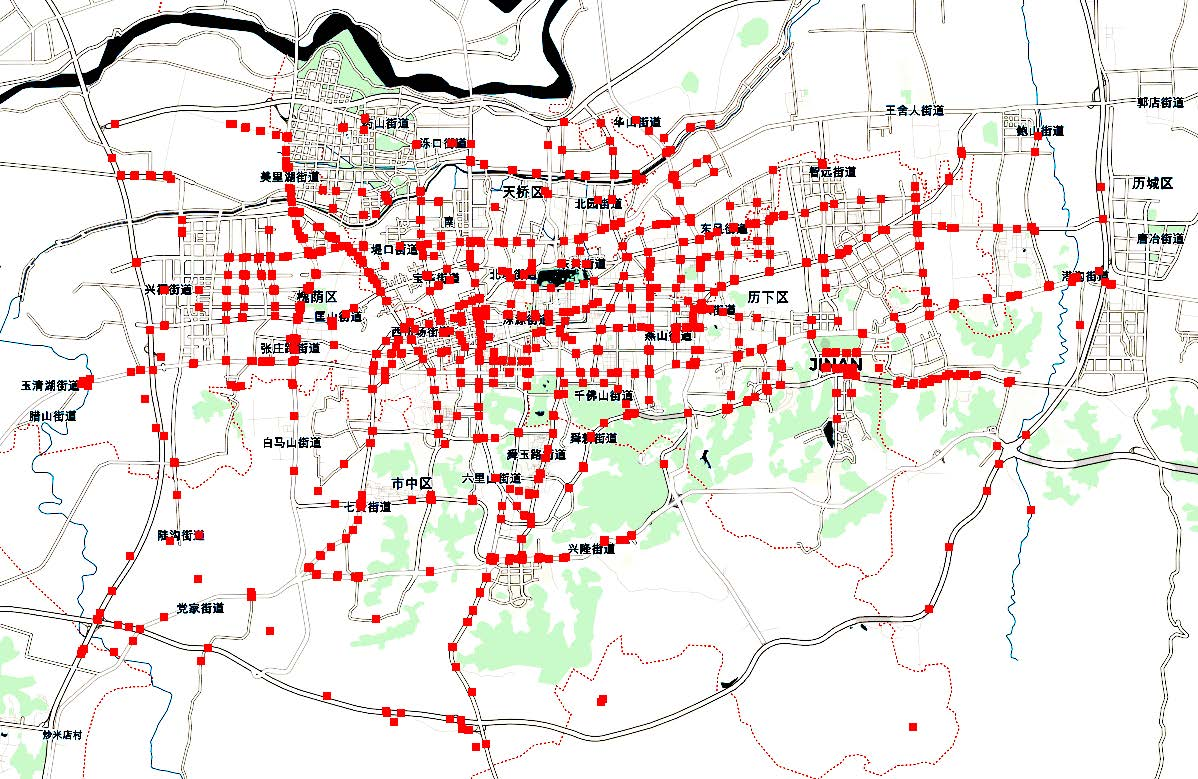
\includegraphics[width=.4\textwidth]{jn.png}
\caption{Traffic surveillance cameras in Jinan, China}
\end{figure}


Nowadays, most traffic lights are still controlled with pre-defined fixed-time plan and are not designed by observing real traffic. Recent studies propose hand-crafted rules according to real traffic data. However, these rules are still pre-defined and cannot be dynamically adjusted w.r.t. real-time traffic.




\section{Related Work}
\quad In this section, we firstly introduce conventional methods for traffic light control, then introduce methods using reinforcement learning.

\subsection{Conventional Traffic Light Control}
\quad Early traffic light control methods can be roughly classified into
two groups. 

The first is pre-timed signal control [6, 18, 23], where a fixed time is determined for all green phases according to historical traffic demand, without considering possible fluctuations in traffic demand. 

The second is vehicle-actuated control methods [5, 20] where the real-time traffic information is used. Vehicle-actuated methods are suitable for the situations with relatively high traffic randomness. 

However, this method largely depends on the hand-craft rules for current traffic condition, without taking into account future situation. Therefore, it cannot reach the global optimal.

\subsection{Reinforcement Learning for Traffic Light Control}
\quad Recently, due to the incapability of dealing with dynamic multi-direction traffic in previous methods, more works try to use re-
inforcement learning algorithms to solve the traffic light control problem [13, 17, 24]. Typically, these algorithms take the traffic on
the road as state, and the operation on light as action. These methods usually show better performance compared with fixed-time
and traffic-responsive control methods.

Methods in [1, 2, 4, 8, 24] designed the state as discrete values like the location of vehicles or number of waited cars. However,
the discrete state-action pair value matrix requires huge storage
space, which keeps these methods from being used in large state
space problems.

To solve the in-managablely large state space of previous meth-
ods, recent studies [15, 22] propose to apply Deep Q-learning meth-
ods using continuous state representations. These studies learn a
Q-function (e.g. a deep neural network) to map state and action to
reward. These works vary in the state representation including hand
craft features (e.g., queue length [15, 17], average delay [10, 22]) and
image features[9, 16, 22]) They are also different in reward design,
including average delay [3, 22],the average travel time [16, 22], and
queue length[15].

However, all these methods assume relatively static traffic en-
vironments, and hence far from the real case. Further, they only
focus on rewards and overlook the adaptability of the algorithms
to the real traffic. Therefore, they cannot interpret why the learned
light signal changes corresponding to the traffic. In this paper, we
try to test the algorithms in a more realistic traffic setting, and add
more interpretation other than reward.

\section{Problem Definition}
\quad Given a traffic scenario, we are supposed to provide a traffic light control plan for the traffic scenario to minimize the average travel time of vehicles.


Traffic light control has attracted a lot of attention in recent years
due to its essential role in adjusting traffic. Current methods gen
erally have two categories, conventional methods, and deep rein
forcement learning based methods. Conventional methods usually
rely on previous knowledge to set fixed time for each light phase
or set changing rules. These rules are prone to dynamically chang
ing traffic. 

Reinforcement learning methods usually take the traffic
condition (e.g., queue length of waiting cars and updated waiting
time) as state, and try to make actions that can improve the traffic
condition based on the current state.

\begin{figure}[H]
\centering
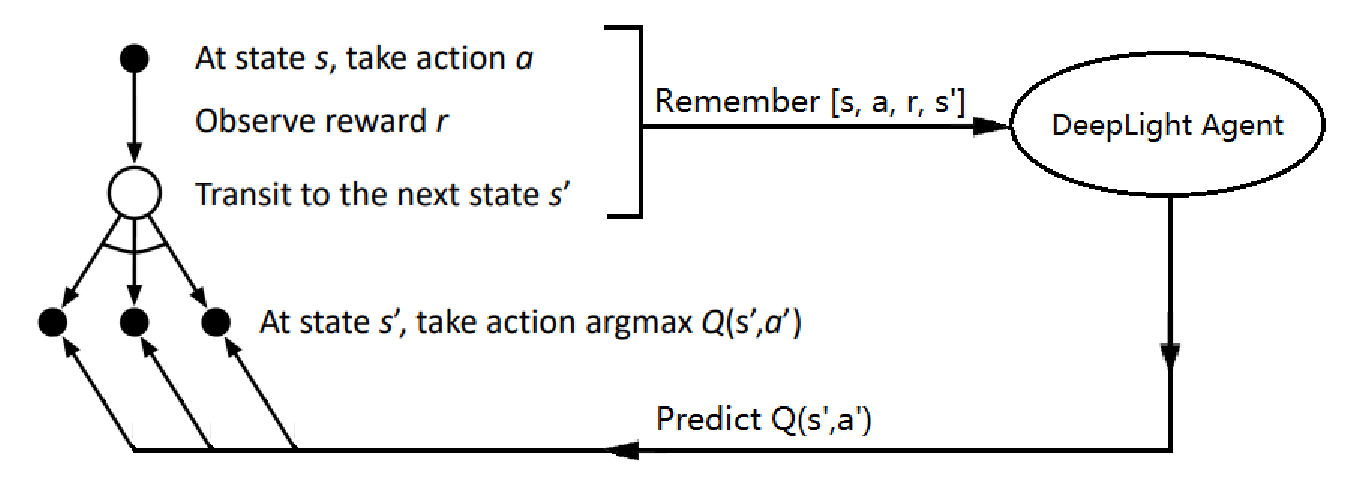
\includegraphics[width=.4\textwidth]{d1.png}
\caption{Problem Abstraction}
\end{figure}

However, the current methods do not consider the complex situ
ations in real case, and hence may lead to stuck in one single kind
of action. This will lead to inferior traffic adjusting performance
under complex traffic situation.
In this section, we propose a deep reinforcement traffic light
agent to solve this problem. 

\section{Agent Design}
\quad First of all , we introduce the state, action and reward representation:
 
 State. Our state is defined for one intersection. For each lane
i at this intersection, the state component includes queue
length $L_i$ , number of vehicles $V_i$ , current phase $P_c$.

Action. Action is defined as next phase $P_n$.

Reward. Reward is defined as a
weighted sum of the following factors:

(1) Sum of queue length L over all approaching lanes, where
L is calculated as the total number of waiting vehicles on
the given lane. A vehicle with a speed of less than 0.1 m/s
is considered as waiting.

(2) Total number of vehicles N that passed the intersection
during time interval $\Delta$t after the last action a.
$$Reward = N - 0.25 L$$

Hence, given the current state s of the traffic condition, the mission
of the agent G is to find the action a (change or keep current phase)
that may lead to the maximum reward r in the long run, following
the Bellman Equation [21]:
$$q(s_t , a, t) = r_{a,t + 1} + \gamma max q(s_{a,t +1} , a' , t + 1)$$

In this situation, the action
value function q for time t is the summation of the reward of the
next timestamp t + 1 and the maximum potential future reward.
Through this conjecture of future, the agent can select action that
is more suitable for long-run reward.

\section{Network Structure}
\quad In order to estimate the reward based on the state, and action, the
agent needs to learn a Deep Q-Network Q(s, a).
In the real-world scenario, traffic is very complex and contain
many different cases need to be considered separately.

In previous studies, due to the simplified design of the model for
approximating Q-function under complex traffic condition, agents
are having difficulties in distinguishing the decision process for
different phases. Therefore, we hereby propose a network structure
that can explicitly consider the different cases explicitly. We call
this special sub-structure “Phase Gate”.

\begin{figure}[H]
\centering
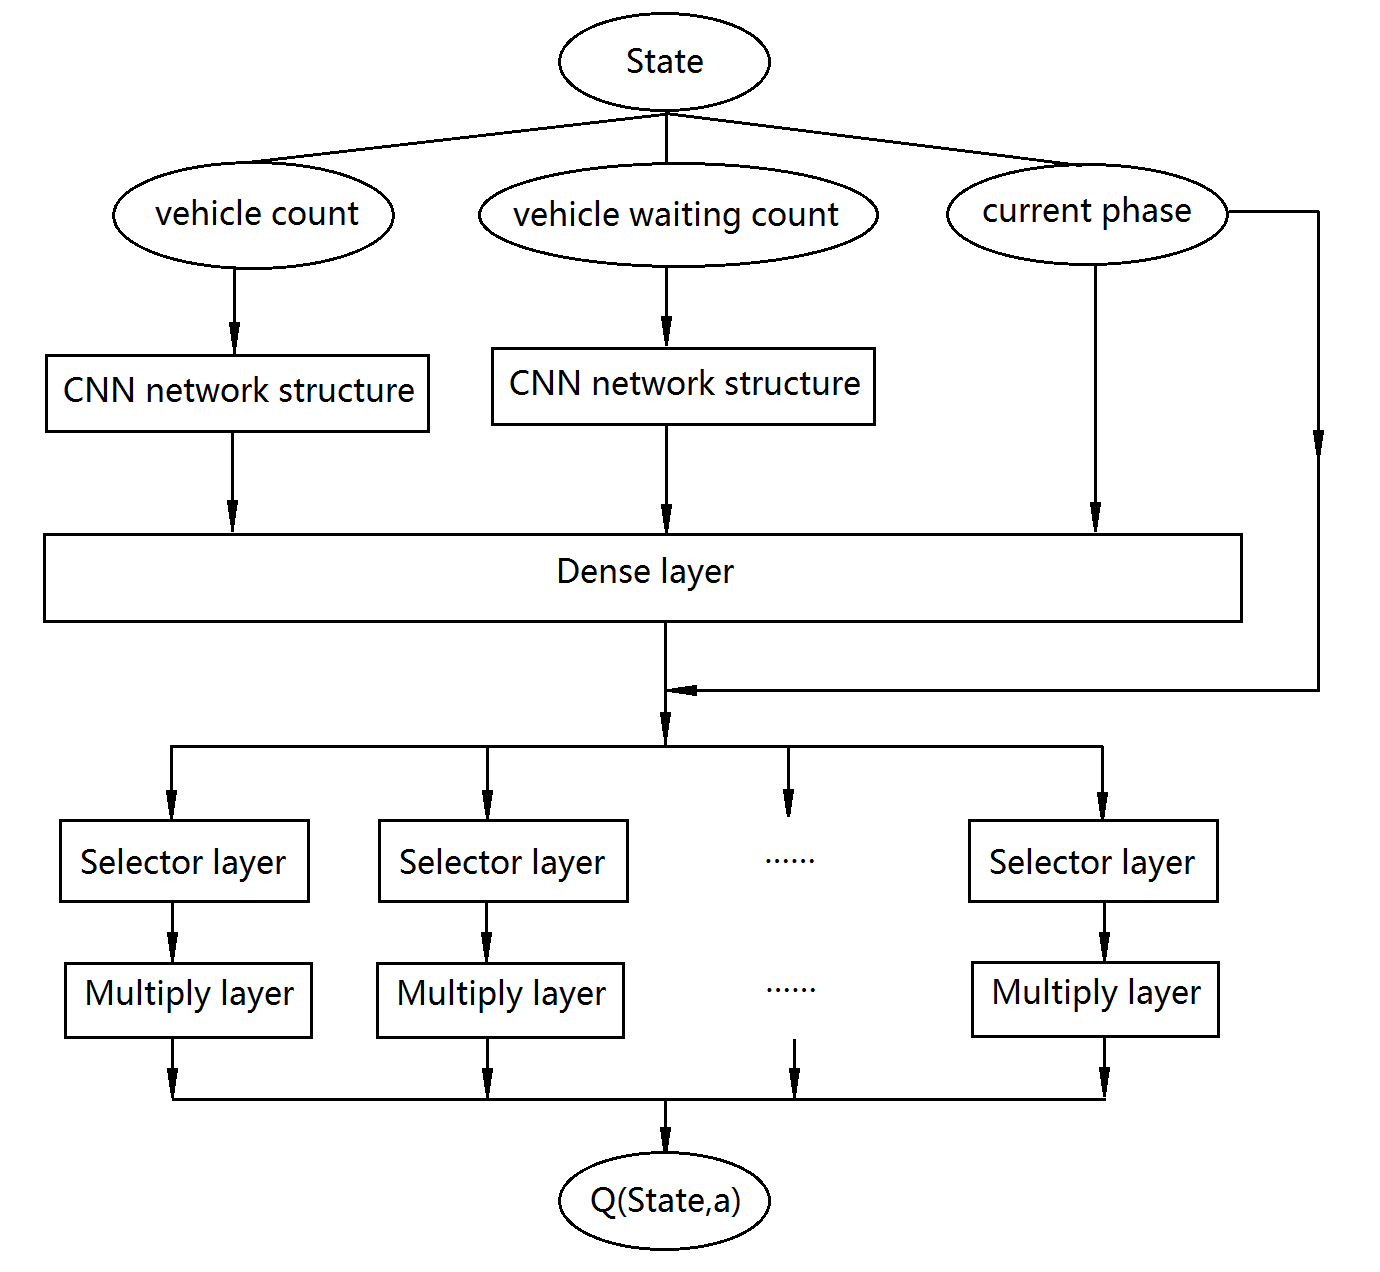
\includegraphics[width=.4\textwidth]{2d.png}
\caption{Eval Net of DQN}
\end{figure}
Our whole network structure can be shown as in Figure 3. The
image features are extracted from the observations of the traffic
condition and fed into two convolutional layers.

The output of these
layers are concatenated with the four explicitly mined features. 
The concatenated features are then fed into
fully-connected layers to learn the mapping from traffic conditions
to potential rewards.

Then, for each phase, we design a separate
learning process of mapping from rewards to the value of making
decisions Q(s, a). These separate processes are selected through a
gate controlled by the phase.  This will distinguish the decision
process for different phases, prevent the decision from favoring
certain action, and enhance the fitting ability of the network.

\section{Memory Palace and Model Updating}

\quad Periodically, the agent will take samples from the memory and use
them to update the network. This memory is maintained by adding
the new data samples in and removing the old samples occasionally.
This technique is noted as experience replay [19] and has been
widely used in reinforcement learning models.

However, in the real traffic setting, traffic on different lanes can
be really imbalanced. As previous methods [9, 10, 15, 22] store all the
state-action-reward training samples in one memory, this memory
will be dominated by the phases and actions that appear most
frequently in imbalanced settings. Then, the agent will be learned to
estimate the reward for these frequent phase-action combinations
well, but ignore other less frequent phase-action combinations.

This will cause the learned agent to make bad decisions on the
infrequent phase-action combinations. Therefore, when traffic on
different lanes are dramatically different, these imbalanced samples
will lead to inferior performance on less frequent situation.
Inspired by Memory Palace theory [11, 14] in cognitive psychol
ogy, we can solve this imbalance by using different memory palaces
for different phase-action combinations. 


\section{Experiments}
\quad In this section, we conduct experiments using both fsy's traffic data. We show a comprehensive quantitative evaluation by comparing with other methods.
\begin{figure}[H]
\centering
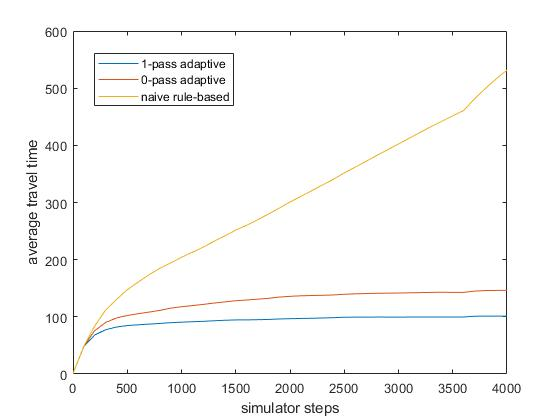
\includegraphics[width=.4\textwidth]{pass.jpg}
\caption{Perfomance of Each Model}
\end{figure}

\section{Extensions to DQN}
\quad DQN has been an important milestone, but several limita-tions of this algorithm are now known, and many extensionshave been proposed. We propose a selection of six exten-sions  that  each  have  addressed  a  limitation  and  improvedoverall performance. To keep the size of the selection man-ageable, we picked a set of extensions that address distinctconcerns (e.g., just one of the many addressing exploration).

\subsection{Double Q-learning}

Conventional Q-learning is affectedby an overestimation bias, due to the maximization step inEquation 1, and this can harm learning. Double Q-learning(van Hasselt 2010), addresses this overestimation by decou-pling, in the maximization performed for the bootstrap tar-get, the selection of the action from its evaluation. It is pos-sible  to  effectively  combine  this  with  DQN  (van  Hasselt,Guez, and Silver 2016), using the loss
$$(R_{t+1}+\gamma {t+1}q_{\theta}(S_{t+1},\text{argmax}_{a'} q_{\theta} (S_{t+1},a')) - q_{theta}(S_t,A_t))^2.$$

This change was shown to reduce harmful overestimationsthat were present for DQN, thereby improving performance.


\subsection{Prioritized replay}
\quad DQN samples uniformly from the re-play  buffer.  Ideally,  we  want  to  sample  more  frequentlythose  transitions  from  which  there  is  much  to  learn.  As  aproxy  for  learning  potential,  prioritized  experience  replay(Schaul et al. 2015) samples transitions with probabilityptrelative to the last encountered absoluteTD error.

\subsection{Dueling networks}
\quad The dueling network is a neural net-work  architecture  designed  for  value  based  RL.  It  fea-tures two streams of computation, the value and advantagestreams, sharing a convolutional encoder, and merged by aspecial aggregator (Wang et al. 2016). 

\subsection{Multi-step learning}
\quad Q-learning accumulates a single re-ward and then uses the greedy action at the next step to boot-strap. Alternatively, forward-viewmulti-steptargets can beused (Sutton 1988).

A multi-step variant of DQN is then defined by minimizingthe alternative loss.Multi-step targets with suitably tunednoften lead to fasterlearning (Sutton and Barto 1998).

\subsection{Distributional RL}
\quad In reinforcement learning an agent interacts with the environment by taking actions and observing the next state and reward. When sampled probabilistically, these state transitions, rewards, and actions can all induce randomness in the observed long-term return. Traditionally, reinforcement learning algorithms average over this randomness to estimate the value function.
    
    We build on recent work advocating a distributional approach to reinforcement learning in which the distribution over returns is modeled explicitly instead of only estimating the mean.
    
    That is, we examine methods of learning the value distribution instead of the value function. We give results that close a number of gaps between the theoretical and algorithmic results given by Bellemare, Dabney, and Munos (2017).
    
    First, we extend existing results to the approximate distribution setting.
    Second, we present a novel distributional reinforcement learning algorithm consistent with our theoretical formulation.
    Finally, we evaluate this new algorithm on the Atari 2600 games, observing that it significantly outperforms many of the recent improvements on DQN, including the related distributional algorithm C51. 

\subsection{Noisy Nets}
\quad The  limitations  of  exploring  using $\epsilon$-greedypolicies are clear in games such as Montezuma’s Revenge,where many actions must be executed to collect the first re-ward.  Noisy  Nets  (Fortunato  et  al.  2017)  propose  a  noisylinear layer that combines a deterministic and noisy stream,$$y =  (b + Wx) + (b_{noisy} \cdot \epsilon^b + (W_{noisy} \cdot \epsilon^w)x),$$ where $\epsilon^b$and $\epsilon^w$ are random variables, and $\cdot$ denotes the element-wise product. This transformation can then be usedin place of the standard lineary=b+Wx. Over time, thenetwork can learn to ignore the noisy stream, but will do soat different rates in different parts of the state space, allowingstate-conditional exploration with a form of self-annealing.

\section{Experimental Methods}
\quad We now describe the methods and setup used for configuringand evaluating the learning agents

\subsection{Evaluation Methodology}
\quad We evaluated all agents on 57Atari  2600  games  from  the  arcade  learning  environment(Bellemare et al. 2013). We follow the training and evalu-ation procedures of Mnih et al. (2015) and van Hasselt et al.(2016). 

The average scores of the agent are evaluated duringtraining, every 1M steps in the environment, by suspendinglearning  and  evaluating  the  latest  agent  for  500K  frames.Episodes  are  truncated  at  108K  frames  (or  30  minutes  ofsimulated play), as in van Hasselt et al. (2016).

Agents’ scores are normalized, per game, so that 0\% cor-responds to a random agent and 100\% to the average scoreof  a  human  expert.  Normalized  scores  can  be  aggre gatedacross all Atari levels to compare the performance of dif-ferent agents. It is common to track themedianhuman nor-malized performance across all games. We also consider thenumber of games where the agent’s performance is abovesome fraction of human performance, to disentangle whereimprovements in the median come from. The mean human normalized performance is potentially less informative, as itis dominated by a few games (e.g., Atlantis) where agents achieve scores orders of magnitude higher than humans do.

Besides tracking the median performance as a function of environment steps, at the end of training we re-evaluate the best agent snapshot using two different testing regimes. Intheno-ops startsregime, we insert a random number (up to30) of no-op actions at the beginning of each episode (as wedo  also  in  training).  In  the human starts regime,  episodesare initialized with points randomly sampled from the initialportion of human expert trajectories (Nair et al. 2015); thedifference between the two regimes indicates the extent towhich the agent has over-fit to its own trajectories.

Due to space constraints, we focus on aggregate results across  games.  However,  in  the  appendix  we  provide  fulllearning curves for all games and all agents, as well as de-tailed comparison tables of raw and normalized scores, inboth the no-op and human starts testing regimes.

\subsection{Hyper Parameter Tuning}

\quad All   Rainbow’s   componentshave  a  number  of  hyper-parameters.  The  combinatorialspace  of  hyper-parameters  is  too  large  for  an  exhaustivesearch,  therefore  we  have  performed  limited  tuning.  Foreach component, we started with the values used in the paperthat introduced this component, and tuned the most sensitiveamong hyper-parameters by manual coordinate descent.DQN and its variants do not perform learning updates dur-ing the first200Kframes, to ensure sufficiently uncorrelatedupdates.  We  have  found  that,  with  prioritized  replay,  it  ispossible to start learning sooner, after only80Kframes.

DQN starts with an exploration of 1, corresponding toacting uniformly at random; it anneals the amount of explo-ration over the first 4M frames, to a final value of 0.1 (low-ered to 0.01 in later variants). Whenever using Noisy Nets,we acted fully greedily , with a value of 0.5 for the $\alpha$ 0 hyper-parameter used to initialize the weights in the noisystream1. 

For agents without Noisy Nets, we used $\epsilon$-greedy but decreased the exploration rate faster than was previouslyused, annealing to 0.01 in the first 250K frames.We  used  the  Adam  optimizer  (Kingma  and  Ba  2014),which  we  found  less  sensitive  to  the  choice  of  the  learn-ing rate than RMSProp. DQN uses a learning rate of $\alpha$=0.00025.

In all Rainbow’s variants we used a learning rateof $\alpha$/4,  selected  among\{$\alpha$/2,$\alpha$/4,$\alpha$/6\},  and  a  value  of1.5*10-4 for Adam’s hyper-parameter.For replay prioritization we used the recommended pro-portional variant, with priority exponent $\omega$ of 0.5, and lin-early increased the importance sampling exponent $\beta$ from 0.4 to 1 over the course of training. The priority exponent $\omega$ was tuned comparing values of\{0.4,0.5,0.7\}. 

Using the KL loss of distributional DQN as priority, we have observedthat performance is very robust to the choice of $\omega$. The  value  of n in  multi-step  learning  is  a  sensitivehyper-parameter of Rainbow. We compared values of n=1,3,and5. We observed that bothn=  3 an d5did wellinitially, but overalln= 3performed the best by the end.The hyper-parameters (see Table 1) are identical acrossall 57 games, i.e., the Rainbow agent really is asingleagentsetup that performs well across all the games.

\section{Conclusion}
\quad In this paper, we address the traffic light control problem using a
well-designed reinforcement learning approach. We conduct exten
sive experiments using both synthetic and real world experiments
and demonstrate the superior performance of our proposed method
over state-of-the-art methods. In addition, we show in-depth case
studies and observations to understand how the agent adjust to
the changing traffic, as a complement to quantitative measure on
rewards. These in-depth case studies can help generate traffic rules
for real world application.

We also acknowledge the limitations of our current approach
and would like to point out several important future directions to
make the method more applicable to real world. First, we can extend
the two-phase traffic light to multi-phase traffic light, which will in
volve more complicated but more realistic state transition. Second,
our paper addresses a simplified one intersection case, whereas
the real world road network is much more complicated than this.

Although some studies have tried to solve the multi-intersection
problem by using multiple reinforcement learning agents, they do
not explicitly consider the interactions between different intersec
tions (i.e., how can the phase of one intersection affect the state of
nearby intersections) and they are still limited to small number of
intersections. Lastly, our approach is still tested on a simulation
framework and thus the feedback is simulated. Ultimately, a field
study should be conducted to learn the real-world feedback and to
validate the proposed reinforcement learning approach.

\section{References}

\quad [1] Monireh Abdoos, Nasser Mozayani, and Ana LC Bazzan. 2013. Holonic multi-
agent system for traffic signals control. Engineering Applications of Artificial
Intelligence 26, 5 (2013), 1575–1587.

[2] Baher Abdulhai, Rob Pringle, and Grigoris J Karakoulas. 2003. Reinforcement
learning for true adaptive traffic signal control. Journal of Transportation Engi-
neering 129, 3 (2003), 278–285.

[3] Itamar Arel, Cong Liu, T Urbanik, and AG Kohls. 2010. Reinforcement learning-
based multi-agent system for network traffic signal control. IET Intelligent
Transport Systems 4, 2 (2010), 128–135.

[4] Bram Bakker, Shimon Whiteson, Leon Kester, and Frans CA Groen. 2010. Traf-
fic light control by multiagent reinforcement learning systems. In Interactive
Collaborative Information Systems. Springer, 475–510.

[5] Seung-Bae Cools, Carlos Gershenson, and Bart D’Hooghe. 2013. Self-organizing
traffic lights: A realistic simulation. In Advances in applied self-organizing systems.
Springer, 45–55.

[6] Francois Dion, Hesham Rakha, and Youn-Soo Kang. 2004. Comparison of delay es-
timates at under-saturated and over-saturated pre-timed signalized intersections.
Transportation Research Part B: Methodological 38, 2 (2004), 99–122.

[7] The Economist. 2014. The cost of traffic jams. https://www.economist.com/blogs/
economist-explains/2014/11/economist-explains-1.

[8] Samah El-Tantawy, Baher Abdulhai, and Hossam Abdelgawad. 2013. Multiagent
reinforcement learning for integrated network of adaptive traffic signal con-
trollers (MARLIN-ATSC): methodology and large-scale application on downtown
Toronto. IEEE Transactions on Intelligent Transportation Systems 14, 3 (2013),
1140–1150.

[9] Juntao Gao, Yulong Shen, Jia Liu, Minoru Ito, and Norio Shiratori. 2017. Adaptive
Traffic Signal Control: Deep Reinforcement Learning Algorithm with Experience
Replay and Target Network. arXiv preprint arXiv:1705.02755 (2017).

[10] Wade Genders and Saiedeh Razavi. 2016. Using a deep reinforcement learning
agent for traffic signal control. arXiv preprint arXiv:1611.01142 (2016).

[11] Robert Godwin-Jones. 2010. Emerging technologies. (2010).

[12] Federico Guerrini. 2014. Traffic Congestion Costs Americans \$124 Billion A Year,
Report Says. Forbes, October (2014).

[13] Lior Kuyer, Shimon Whiteson, Bram Bakker, and Nikos Vlassis. 2008. Multia-
gent reinforcement learning for urban traffic control using coordination graphs.
Machine learning and knowledge discovery in databases (2008), 656–671.

[14] Eric LG Legge, Christopher R Madan, Enoch T Ng, and Jeremy B Caplan. 2012.
Building a memory palace in minutes: Equivalent memory performance using
virtual versus conventional environments with the Method of Loci. Acta psycho-
logica 141, 3 (2012), 380–390.

[15] Li Li, Yisheng Lv, and Fei-Yue Wang. 2016. Traffic signal timing via deep rein-
forcement learning. IEEE/CAA Journal of Automatica Sinica 3, 3 (2016), 247–254.

[16] Mengqi Liu, Jiachuan Deng, Ming Xu, Xianbo Zhang, and Wei Wang. 2017.
Cooperative Deep Reinforcement Learning for Tra ic Signal Control. (2017).

[17] Patrick Mannion, Jim Duggan, and Enda Howley. 2016. An experimental re-
view of reinforcement learning algorithms for adaptive traffic signal control. In
Autonomic Road Transport Support Systems. Springer, 47–66.

[18] Alan J Miller. 1963. Settings for fixed-cycle traffic signals. Journal of the Opera-
tional Research Society 14, 4 (1963), 373–386.

[19] Volodymyr Mnih, Koray Kavukcuoglu, David Silver, Andrei A Rusu, Joel Veness,
Marc G Bellemare, Alex Graves, Martin Riedmiller, Andreas K Fidjeland, Georg
Ostrovski, et al. 2015. Human-level control through deep reinforcement learning.
Nature 518, 7540 (2015), 529.

[20] Isaac Porche and Stephane Lafortune. 1999. Adaptive look-ahead optimization of
traffic signals. Journal of Intelligent Transportation System 4, 3-4 (1999), 209–254.

[21] Richard S Sutton and Andrew G Barto. 1998. Reinforcement learning: An intro-
duction. Vol. 1. MIT press Cambridge.

[22] Elise van der Pol and Frans A Oliehoek. 2016. Coordinated Deep Reinforcement
Learners for Traffic Light Control. NIPS.

[23] F. V Webster. 1958. Traffic signal settings. Road Research Technical Paper 39
(1958).

[24] MA Wiering. 2000. Multi-agent reinforcement learning for traffic light control.
In Machine Learning: Proceedings of the Seventeenth International Conference
(ICML’2000). 1151–1158.

\end{document}
